
\documentclass[a4paper,12pt]{article}
\usepackage[utf8]{inputenc}
\usepackage[a4paper,
            bindingoffset=0.2in,
            left=1in,
            right=1in,
            top=1in,
            bottom=1in,
            footskip=.25in]{geometry}


%###############################################################################

%\input{~/layout/global_layout}


%###############################################################################

% packages begin

\usepackage[
  backend=biber,
  sortcites=true,
  style=alphabetic,
  eprint=true,
  backref=true
]{biblatex}
\addbibresource{bibliography.bib}

\usepackage{euscript}[mathcal]
% e.g. \mathcal{A} for fancy letters in mathmode
\usepackage{amsmath,amssymb,amstext,amsthm}

\usepackage{mdframed}
\newmdtheoremenv[nobreak=true]{problem}{Problem}[subsection]
\newmdtheoremenv[nobreak=true]{claim}{Claim}[subsection]
\newtheorem{definition}{Definition}[subsection]
\newtheorem{lemma}{Lemma}[claim]
\newtheorem{plemma}{Lemma}[problem]

\usepackage{mathtools}
\DeclarePairedDelimiter\ceil{\lceil}{\rceil}
\DeclarePairedDelimiter\floor{\lfloor}{\rfloor}

\usepackage{enumerate}
\usepackage[pdftex]{graphicx}
\usepackage{subcaption}
% 'draft' für schnelleres rendern mitübergeben -> [pdftex, draft]
% dadruch wird nicht das bild mitgerendered, sondern nur ein kasten mit bildname -> schont ressourcen

\usepackage{hyperref}

\usepackage{tikz}
\usetikzlibrary{arrows,automata,matrix,positioning,shapes}

% for adding non-formatted text to include source-code
\usepackage{listings}
\lstset{language=Python,basicstyle=\footnotesize}
% z.B.:
% \lstinputlisting{source_filename.py}
% \lstinputlisting[lanugage=Python, firstline=37, lastline=45]{source_filename.py}
%
% oder
%
% \begin{lstlisting}[frame=single]
% CODE HERE
%\end{lstlisting}
\usepackage{algorithm}
\usepackage{algpseudocode}

\usepackage{wasysym}

\usepackage{titling}
\usepackage{titlesec}
\usepackage[nocheck]{fancyhdr}
\usepackage{lastpage}

\usepackage{kantlipsum}
\usepackage[colorinlistoftodos,prependcaption,textsize=tiny]{todonotes}

% packages end
%###############################################################################

\pretitle{% add some rules
  \begin{center}
    \LARGE\bfseries
} %, make the fonts bigger, make the title (only) bold
\posttitle{%
  \end{center}%
  %\vskip .75em plus .25em minus .25em% increase the vertical spacing a bit, make this particular glue stretchier
}
\predate{%
  \begin{center}
    \normalsize
}
\postdate{%
  \end{center}%
}

\titleformat*{\section}{\Large\bfseries}
\titleformat*{\subsection}{\large\bfseries}
\titleformat*{\subsubsection}{\normalsize\bfseries}

\titleformat*{\paragraph}{\Large\bfseries}
\titleformat*{\subparagraph}{\large\bfseries}

%###############################################################################
% TODO define Headers and Fotter

\pagestyle{fancy}
\fancyhf{}
% l=left, c=center, r=right; e=even_pagenumber, o=odd_pagenumber; h=header, f=footer
% example: [lh] -> left header, [lof,ref] -> fotter left when odd, right when even
%\fancyhf[lh]{}
%\fancyhf[ch]{}
%\fancyhf[rh]{}
%\fancyhf[lf]{}
\fancyhf[cf]{\footnotesize Page \thepage\ of \pageref*{LastPage}}
%\fancyhf[rf]{}
\renewcommand{\headrule}{} % removes horizontal header line

% Fotter options for first page

\fancypagestyle{firstpagestyle}{
  \renewcommand{\thedate}{\textmd{}} % removes horizontal header line
  \fancyhf{}
  \fancyhf[lh]{\ttfamily M.Sc. Computer Science\\KTH Royal Institute of Technology}
  \fancyhf[rh]{\ttfamily Period 3\\\today}
  \fancyfoot[C]{\footnotesize Page \thepage\ of \pageref*{LastPage}}
  \renewcommand{\headrule}{} % removes horizontal header line
}
%###############################################################################
% Todo: define Title

\title{
  \normalsize{DD2358 VT25 Introduction to}\\
  \normalsize{High Performance Computing}\\
  \large{Assignment 4 -- Optimization with Parallelization}\\
}
\author{
  \small Rishi Vijayvargiya\\[-0.75ex]
%  \footnotesize\texttt{MN: }\\[-1ex]
  \scriptsize\texttt{rishiv@kth.se}
  \and
  \small Lennart Herud\\[-0.75ex]
%  \footnotesize\texttt{MN: }\\[-1ex]
  \scriptsize\texttt{herud@kth.se}
  \and
  \small Paul Mayer\\[-0.75ex]
%  \footnotesize\texttt{MN: }\\[-1ex]
  \scriptsize\texttt{pmayer@kth.se}
  \and
  \small Adrian Sušec\\[-0.75ex]
%  \footnotesize\texttt{MN: }\\[-1ex]
  \scriptsize\texttt{susec@kth.se}
}
\date{}

%###############################################################################
% define Commands

\newcommand{\N}{\mathbb{N}}
\newcommand{\R}{\mathbb{R}}
\newcommand{\Z}{\mathbb{Z}}
\newcommand{\I}{\mathbb{I}}

\newcommand{\E}{\mathbb{E}}
\newcommand{\Prob}{\mathbb{P}}

\renewcommand{\epsilon}{\varepsilon}

% Todo: Set Counter to Excercise Sheet Number
%\setcounter{section}{1}
%\setcounter{subsection}{1}

%###############################################################################
%###############################################################################

\begin{document}
\maketitle
\thispagestyle{firstpagestyle}

% \tableofcontents
\listoftodos

\vspace{1em}

%---
%
\section*{Prefix}
\todo[inline]{Make sure title and headers are correctly changed!}
\todo[inline]{Change counter to match excercise sheet}

% content begin
%

\section{Code Repository}
The code for this assignment can be found in the following github repository: \url{https://github.com/paulmyr/DD2358-HPC25/tree/master/04_parallel}.

\section{Wildfire Spread in Parallel}
\section{Bonus: Ocean Circulation with Dask}
The code and associated files for the bonus section can be found under the \verb|bonus/| directory of the repository, here: \url{https://github.com/paulmyr/DD2358-HPC25/tree/master/04_parallel/bonus}. The original code provided to us can be found in the \verb|ocean_deafult.py| file -- with some augmentation to help with profiling and testing against the Dask implementation.

\subsection{Dask Implementation}

\subsubsection{Brief Explanation}
To parallelize the provided code with Dask, we utilized the \verb|map_overlap| function of the Dask arrays to \textit{schedule} the parallel updates to our 3 arrays -- \verb|u_velocity|, \verb|v_velocity|, and \verb|temperature|. The Dask-parallelized implementation can be found in the \verb|ocean_dask.py| file in the repository.

We first converted all the grids used in the ocean updates from \verb|numpy| arrays to Dask arrays using the \verb|da.from_array| function with a specified chunk size (in the report, \verb|da| refers to \verb|dask.array|). 

Then for clarity, we created 2 separate \verb|update| functions for the changes to the velocity and to the temperature grids. Then, we passed in these functions as the first argument to \verb|map_overlap|. This was followed by the arguments that the function 2 \verb|update| functions accept. For the \verb|depth| argument of the \verb|map_overlap| function, we used the value of 1, since that is all that was required in the overalpping computation performed by the laplacian calculation through the \verb|np.roll| operation. Finally, the \verb|boundary| was set to be \verb|periodic| -- since that seems to give the correct and intended output when compared with the default serial implementation. With this, the edges \textit{wrap around}, which we believe was the requirement to correctly compute the laplacian. The snippet below from \verb|ocean_dask.py| illustrates this:

\begin{lstlisting}[language=python,basicstyle=\tiny\ttfamily]
# ... other code
        u_velocity = da.map_overlap(update_velocity, u_velocity, wind, depth=1, boundary="periodic", dtype=da.float64)
        v_velocity = da.map_overlap(update_velocity, v_velocity, wind, depth=1, boundary="periodic", dtype=da.float64)
        temperature = da.map_overlap(update_temp, temperature, depth=1, boundary="periodic", dtype=da.float64)
# ... other code

\end{lstlisting}
The code above would then build a \textit{task graph} which would apply the updates (and the laplacian operation that is required to perform the updates) to grid partitions in parallel, instead of working on entire grids in one go. This was performed in a loop for the desired number of iterations. 

However, \textit{nothing was computed here} -- since Dask was only building a computation task graph at this point (as explained in a recent \href{https://canvas.kth.se/courses/52247/discussion_topics/452810}{Canvas announcement}). To get the actual \textit{result} of the computations, we then call the \verb|compute()| function on each of \verb|u_velocity|, \verb|v_velocity|, and \verb|temperature| Dask arrays \textbf{\underline{after}} the loop, and then return the result. As stated above, this entire code can be found in the \verb|ocean_dask.py| file.

\subsubsection{Correctness Verification}
To ensure that the Dask implementation returns the same result as the default, we implemented some sanity-check unit tests in the \verb|ocean_test.py| file. These are parameterized tests that run the ocean update simulations for 3 different numbers, testing that Dask implementation returns the correct answer for 3 different chunk sizes. We set the same seed in the Dask and the default implementation to ensure that the starting grids are the same. 

All 9 of these tests pass.

\subsubsection{Runtime Comparison}
We compared the running times of the default implementation against the Dask implementation with different chunk-sizes ($50 \times 50, 100 \times 100, 200 \times 200$). The code for this time profiling can be found in the \verb|ocean_profile.py| file. The following observations were obtained on a 2021 M1 MacBook Pro (16 inch), the specifications for which can be found \href{https://support.apple.com/en-us/111901}{here}

We compared the running times of 4 versions of the simulation, where each version was run for 100, 200, 400, and 800 iterations. For each run, the runtime recorded was an average over 5 runs of the simulation. For the default python implementation, only the running time of the \verb|for| loop was recorded. For the Dask implementation, the running time of the \verb|for| loop (where the task graph is created) and of the 3 compute calls on the Dask arrays (where the actual computation is performed) was recorded. The code demarcating which portion of the simulation was timed can be found in the \verb|ocean_default.py| and the \verb|ocean_dask.py| files, in the \verb|run_simulation_default| and the \verb|run_simulation_dask| functions, respectively.

With this setup, we observed the following running times textual format: 

\begin{lstlisting}[language=bash,basicstyle=\tiny\ttfamily]
$ python3 ocean_profile.py
PROFILING COMPUTATION FOR DEFAULT IMPLEMENTATION (runs=5)
Avg Time for 100 iterations: 0.034803566599293845 s 
Avg Time for 200 iterations: 0.06937524999957531 s 
Avg Time for 400 iterations: 0.13857185839951852 s 
Avg Time for 800 iterations: 0.27716657480050344 s 
PROFILING COMPUTATION FOR DASK IMPLEMENTATION (chunk_size=50, runs=5)
Avg Time for 100 iterations: 6.83086175799981 s 
Avg Time for 200 iterations: 14.691950425000687 s 
Avg Time for 400 iterations: 32.8788943749998 s 
Avg Time for 800 iterations: 77.39897956659988 s 
PROFILING COMPUTATION FOR DASK IMPLEMENTATION (chunk_size=100, runs=5)
Avg Time for 100 iterations: 2.7626196668003105 s 
Avg Time for 200 iterations: 6.482563008401485 s 
Avg Time for 400 iterations: 15.559239650000382 s 
Avg Time for 800 iterations: 41.137253450201385 s 
PROFILING COMPUTATION FOR DASK IMPLEMENTATION (chunk_size=200, runs=5)
Avg Time for 100 iterations: 1.6673615167994285 s 
Avg Time for 200 iterations: 3.9416711081998073 s 
Avg Time for 400 iterations: 10.363534933399205 s 
Avg Time for 800 iterations: 30.311092333000126 s 
$
\end{lstlisting}

And this is a graph which visualizes the same values recorded above

\begin{figure}[H]
  \centering
  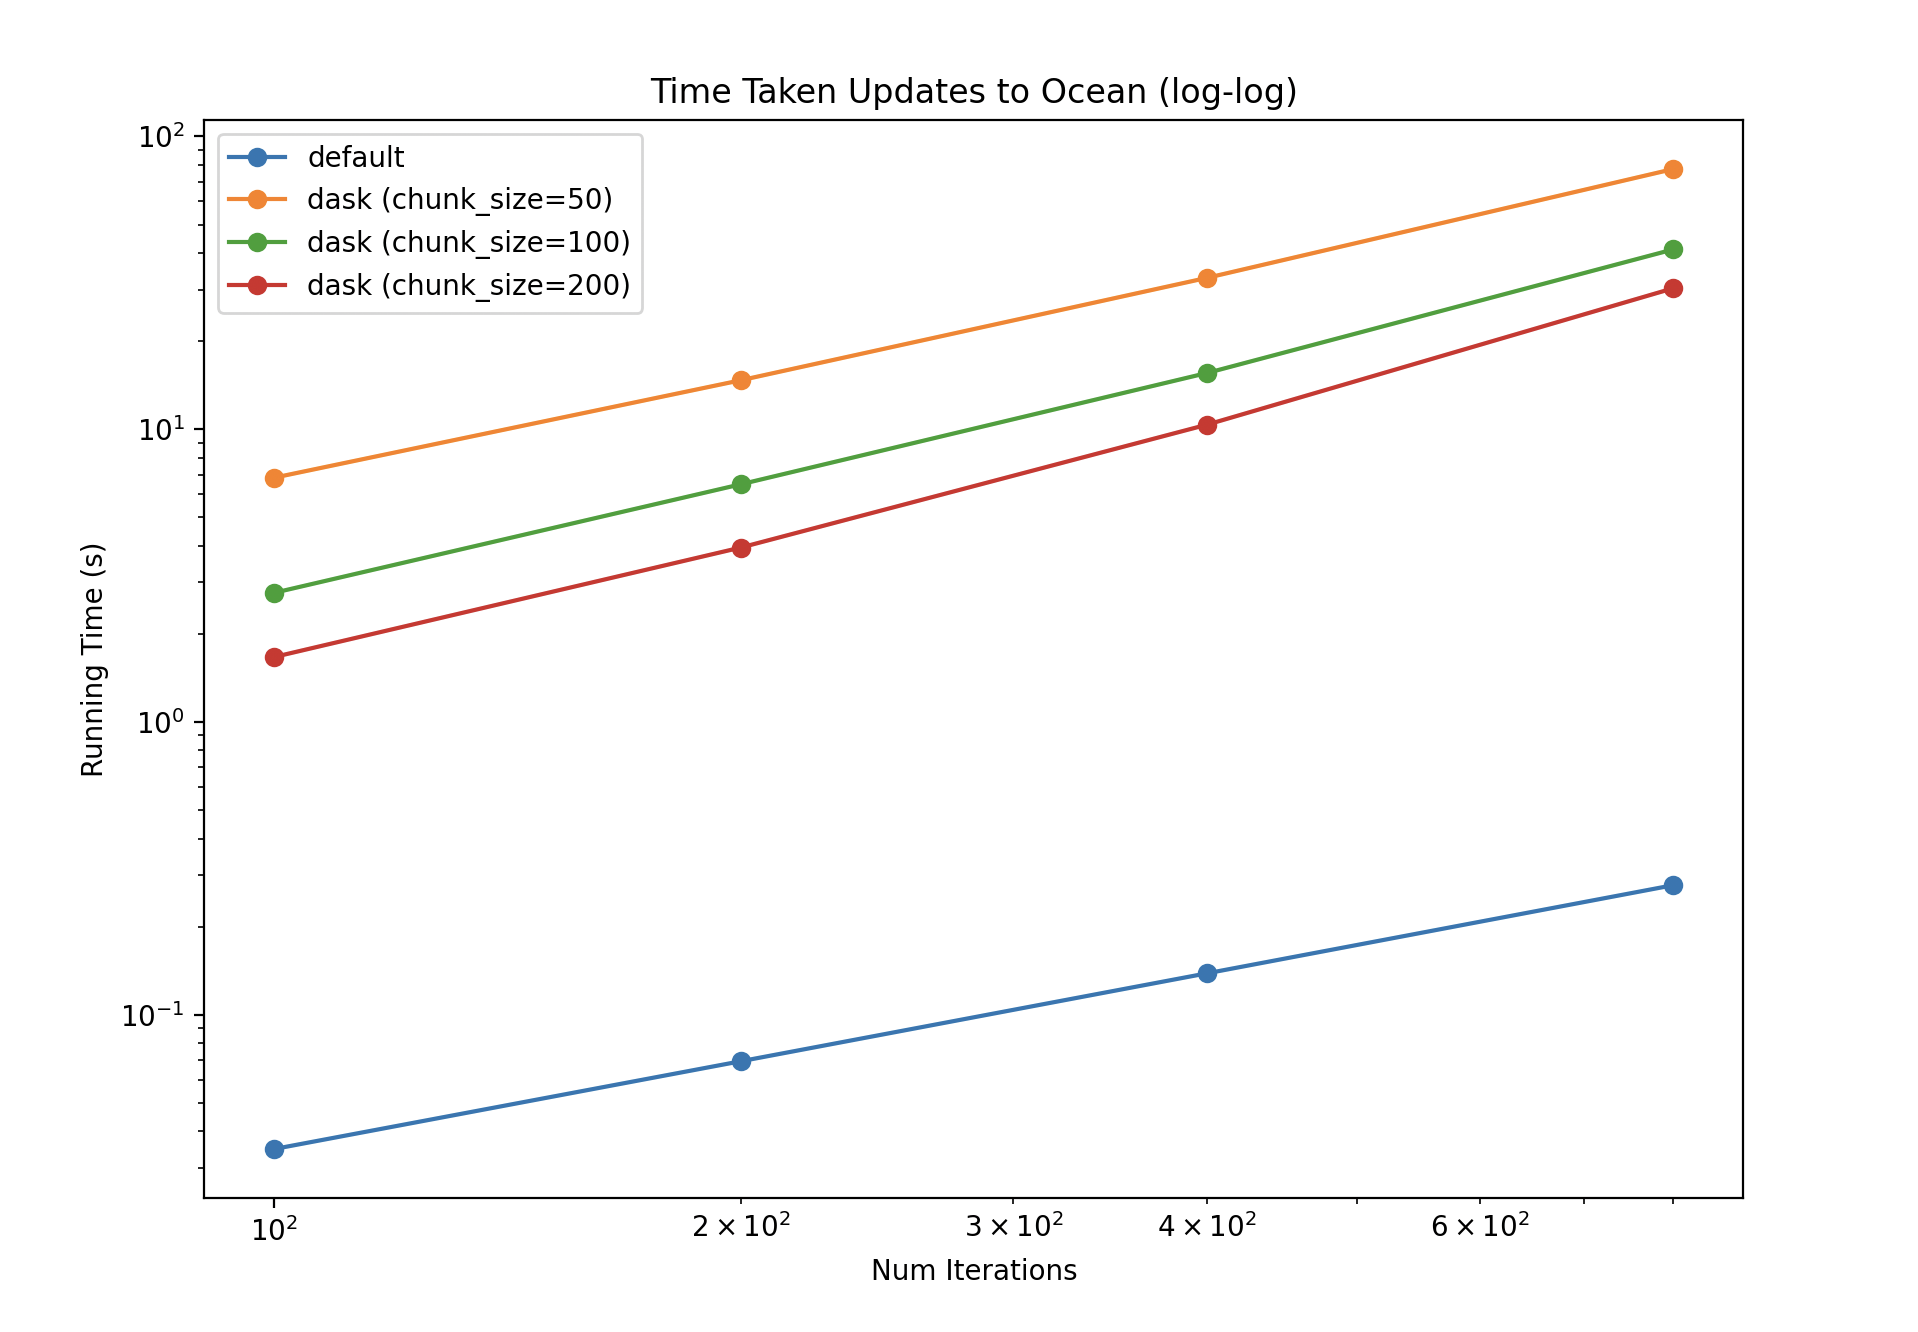
\includegraphics[width=0.8\textwidth]{../images/bonus_default_dask_runtimes.png}
  \caption{Running Time Comparisons For Dask and Default Ocean Updates}
\end{figure}



The first thing that stands out is that the \textbf{default (numpy) implementation outperforms Dask} implementations for all 3 chunk sizes. We believe that this can largely be attributed to the fact that Dask parallelization with the help of \verb|map_overlap| has the overhead of chunk creation, ghost cell management, appropriate wrapping around boundaries (for the \verb|periodic| boundary type), etc. On top of this, Dask needs to manage the intermediate task graphs, creating scheduling workloads with a scheduler, among other things. Additionally, Dask also seems to assume that the underlying memory infrastructure is not one that uses shared-memory, and thus communicates between the different chunks that are created (as explained \href{https://canvas.kth.se/courses/52247/discussion_topics/452810}{here}). 

All these are things that are do not impact the default \verb|numpy| implementation. Thus, to us it appears that there are \textbf{\underline{no advantages in terms of runtime}} of parallelizing this computation using Dask and \verb|map_overlap| on a \underline{shared-memory architecture}, such as the 2021 M1 laptop. 

The second thing to note here is that for the Dask runtimes, the \textbf{smaller the size of the chunk, the worse the runtime}. This agrees with our expectations. Having smaller chunk sizes would in turn mean having more chunks -- which would then lead to more communication between chunks that was discussed above. This would then add to the overhead of using Dask, and would thus increase the runtime. This is exactly what seems to occur in practice as well -- with $50 \times 50$ chunks being the worst, and $200 \times 200$ chunks being the best when it comes to Dask runtimes. 

Finally, for completeness, we would also like to note the trivial observation that the runtime increases across all implementations as the number of iterations increase, as expected. 

\subsection{Performance Monitoring using Dask Dashboard}

\subsubsection{Task Stream \& Worker Monitoring}

\subsubsection{Experiment with Different Chunk Sizes}

\subsubsection{Miscellenaeous Questions}

\begin{itemize}
\item \textbf{\underline{How well-balanced were the worker loads?}}
\item \textbf{\underline{Did any worker run out of memory?}}
\item \textbf{\underline{Was thre idle time or task queueing?}}
\end{itemize}

\subsubsection{VTK Files and Paraview}


% content end
%###############################################################################

% TODO: bibliograpghy when needed
% \printbibliography

\end{document}
